
Chen, St\aa{}rner and Masri performed at Sydney University a detailed experimental investigation of a turbulent evaporating jet of acetone, see \cite{chen}. Droplet diameter, droplet velocity, droplet number density and liquid volumetric flux were measured using a two-component phase Doppler interferometry (PDI) and acetone vapor mass flux was measured using planar laser-induced fluorescence (PLIF).

The experiment consists of a spray nozzle centered on the exit plane of a wind tunnel with 150mm by 150mm that supplies a co-flowing air stream, see Figure \ref{spray_jet}. 
Inside the nozzle, a pressurized liquid jet is surrounded by a carrier air flow until the nozzle exit. The co-flow has a low turbulence intensity of less than $2\%$, so that the effect on the spray jet turbulence is negligible. The main benefit of this setup is the avoidance of flow recirculation near the nozzle exit, what would be an extra complication for the boundary conditions of a numerical simulation.

Acetone evaporation takes place even before the nozzle exit, cooling both the gas and the droplets. The exit temperature shown in Table \ref{table: experiment} was not measured, but computed from energy conservation based on the measurement of acetone vapor mass flux and  the assumption of thermal equilibrium.

\begin{notation}
Sauter mean diameter - SMD or $D_{32}$ - is an average droplet diameter given by:
\begin{equation}
 SMD= \frac{\sum_{droplets} D^3}{\sum_{droplets} D^2} \, .
\end{equation}
\end{notation}

\begin{table}
\centering
 \begin{tabular}{lc}
\hline
Experiment  Data & \\ \hline
Liquid Phase & Acetone \\
Liquid Flow rate at nozzle exit $(g/min)$  &  $7.0$ \\
Carrier air flow rate $(g/min)$ & $135$ \\
Vapor flux at nozzle exit $(g/min)$ & $5.0$ \\
SMD at nozzle exit $(\mu m)$ & $13.7$ \\
Gas temperature at nozzle exit $(K)$ & $280$ \\ 
Gas jet Reynolds Number $(Re=4 \dot{m}_g/\pi D_{nozzle} \mu_g)$ & $16,300$ \\
\hline
 \end{tabular}
\caption{Basic information about the experiment of Chen, St\aa{}rner and Masri, \cite{chen}.}
\label{table: experiment}
\end{table} 


\begin{figure}[!htb]
 \centering
 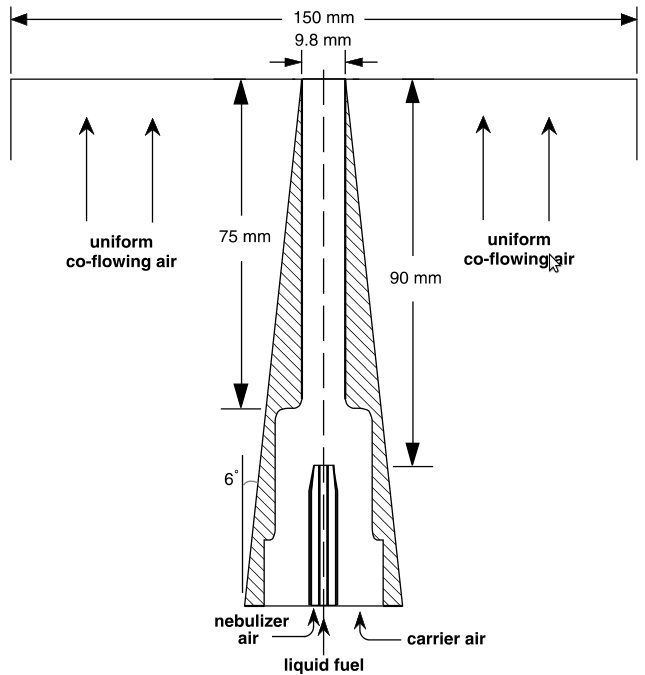
\includegraphics[width=0.4\textheight]{./figuras/chap3/setup.png}
 \caption{Configuration of the spray jet nozzle from \cite{chen}.}
 \label{spray_jet}
\end{figure}

\FloatBarrier
 \section[Boundary Conditions for the Numerical Simulation]{Determining the Boundary Conditions for the Numerical Simulation}

In this section, the boundary conditions for the numerical simulation are obtained from the evailable experimental data. The measurements provide almost complete data for establishing the boundary conditions and few assumptions had to be made.
The list of conditions to be specified for each phase is summarized below.

\subsection{Nozzle}

Below, the boundary conditions at nozzle exit.

\subsubsection{Liquid Phase:}

\begin{description}
  \item[Diameter ($D$):] 
  
The parcel diameter is sampled from a statical distribution built from measurements. \cite{chen} does not provide such measurements at the nozzle exit plane, but only the Sauter mean diameter.  A Lognormal distribution was then specified with $\mu = 10\ \mu m$ and $\sigma=5.5\ \mu m$.

\begin{equation}
 cpf(d; \mu, \sigma) = \frac12 \operatorname{erfc}\!\left[-\frac{\ln D - \mu}{\sigma\sqrt{2}}\right] = \Phi\bigg(\frac{\ln D - \mu}{\sigma}\bigg) \, ,
\end{equation}

\begin{equation}
 pdf(D;\mu,\sigma) = \frac{1}{D \sigma \sqrt{2 \pi}}\, e^{-\frac{(\ln D - \mu)^2}{2\sigma^2}} \, .
\end{equation}

Figure \ref{fig: lognormal} shows the distribution shape. The correspondent Sauter mean diameter is $SMD =14\ \mu m$.
\begin{figure}[!htb]
\centering
  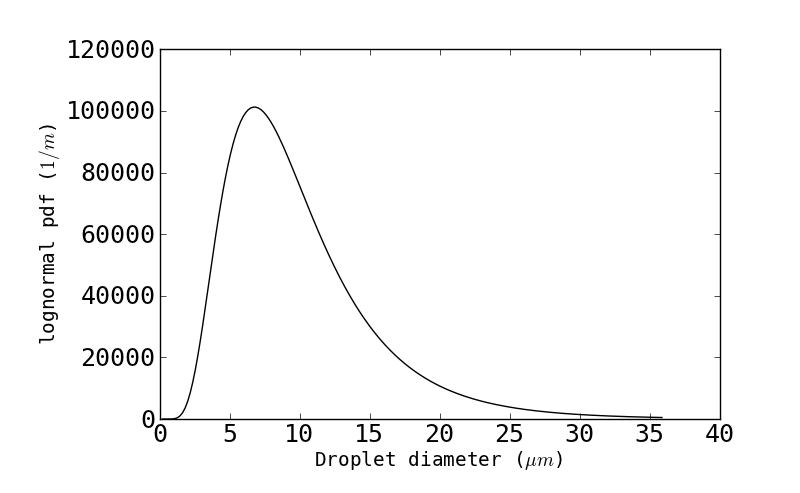
\includegraphics[width=0.75\textwidth]{./figuras/chap3/lognormal.png}
\caption{Lognormal probability density function used for sampling droplet diameter at nozzle exit.}
\label{fig: lognormal}
\end{figure} 
  
\item[Position ($\bv{x}_d$):]
The droplets are inserted in the domain with an aleatory radial coordinate in the interval going from the nozzle axis to the nozzle external radius $(y \in [0, 4.9] \ mm )$, which is sampled for each parcel injection. 
  
  
  \item[Velocity ($\bv{U}_d$):]
  The droplet injection velocity was made dependent only on the injection position according to Figure \ref{fig: bc_dropU}.
  
  \begin{figure}[h]
  \centering
  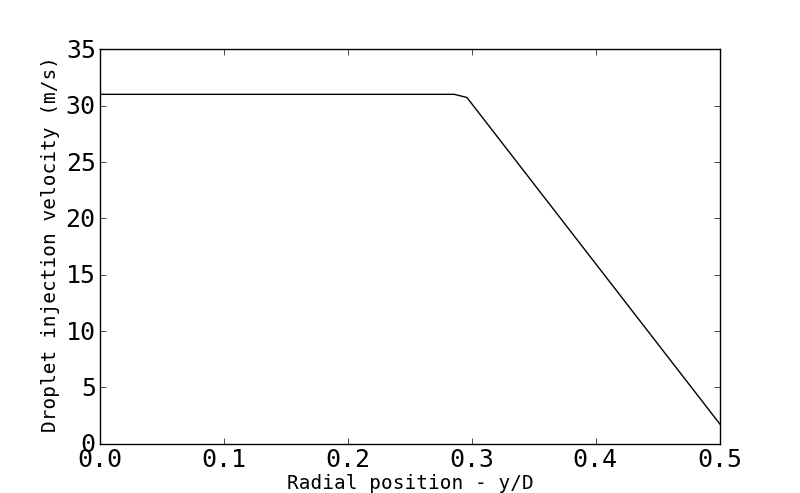
\includegraphics[width=0.65\textwidth]{./figuras/chap3/bc/bc_dropU.png}
  \caption{Droplet injection velocity as a function of its injection position.}
  \label{fig: bc_dropU}
  \end{figure} 
  
  \item[Temperature ($T_d$):] The temperature was determined by assuming thermal equilibrium in the nozzle exit for given mass flow rates of liquid, air and acetone vapor:
  \begin{equation}\label{eq: bc_est_T}
  T_{nozzle}=T_{\infty} - \frac{\dot{m}_{ac} L_{v}}{\dot{m}_g c_{p,g}+\dot{m}_l c_{p,l}} = 280\ K
  \end{equation}
  where $T_{\infty}$ is the ambient temperature and $L_v$ is the latent heat of vaporization of acetone.
  
  The fixed value of $280\ K$ is specified for droplet and gas temperature. 
  
  \item[Mass flow rate ($\dot{m}_d$):] According to the measurements, the liquid mass flow rate is $\dot{m}_d=2\ g/min$.  The parcel injection rate was $5\times10^5\ parcels/s$, yelding about 35,000 parcels in the computational domain.
  \end{description}
  
\subsubsection{Gas Phase:}
  
\begin{description}
  \item[Velocity ($\tilde{\bv{U}}_{nozzle}(\bv{x})$), Turbulent KE ($k_{nozzle}(\bv{x})$) and Dissipation Rate ($\epsilon_{nozzle}(\bv{x})$):] The droplet velocity was obtained from a gas phase only numerical simulation of the nozzle interior with fixed mass flow rate of $\dot{m}_g = 140 g/min$. The turbulence properties in the nozzle inlet was estimated using the following relations from \cite{luppes}:
  \begin{equation}
  k=\frac{3}{2} i^2 \bar{U}_{nozzle}^{2}\, , \quad \epsilon = \frac{c_{\mu}^{3/4} k^{3/2}}{l_m} \, ,
  \end{equation}
  where $\bar{U}_{nozzle}$ is the average velocity inside the nozzle, $i=0.03$ and $l_m = 0.07 D_{nozzle}$.
  The resulting velocity profile was then compared to the mean velocity of the smallest droplets showing good agreement in Figure \ref{fig: bc_gas}.
  
  \item[Temperature ($\tilde{T}_{nozzle}$):] As explained in the liquid phase section, the fixed value of $280\ K$ was used.
  \item[Species Concentration ($\tilde{Y}_{k,nozzle}$):] Given the measured mass flow rates of air ($\dot{m}_{air}$) and acetone vapor ($\dot{m}_{ac}$):
  \begin{equation}
  \begin{split}
  Y_{ac} &= \frac{\dot{m}_{ac}}{\dot{m}_{ac}+\dot{m}_{air}}=0.0357 \, , \\
  Y_{O2} &= 0.233\left( 1- Y_{ac} \right)=0.224 \, , \\
  Y_{N2} &= 1- Y_{ac}-Y_{O2}=0.740 \, .
   \end{split}
  \end{equation}
  \item[Dynamic Pressure ($p_{d,nozzle}$):] A zero gradient condition was used.
\end{description}


\begin{figure}[!htb]
 \centering
\begin{tabular}{cc}
 \subfloat[]{\label{fig: bc_Ux}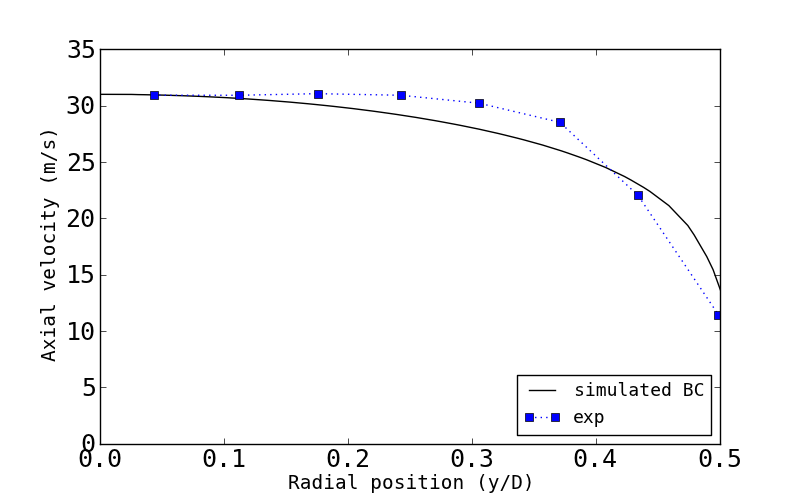
\includegraphics[width=0.5\textwidth]{./figuras/chap3/bc/bc_Ux.png}} &  \subfloat[]{\label{fig: bc_k}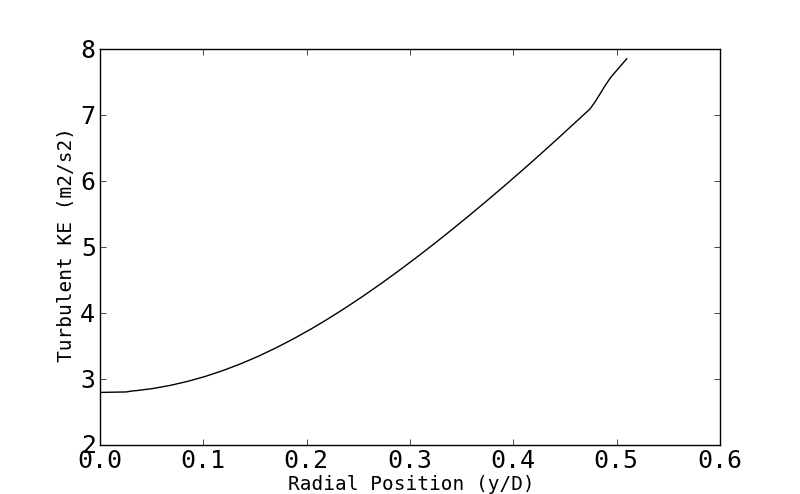
\includegraphics[width=0.5\textwidth]{./figuras/chap3/bc/bc_k.png}} \\
  \subfloat[]{\label{fig: bc_eps}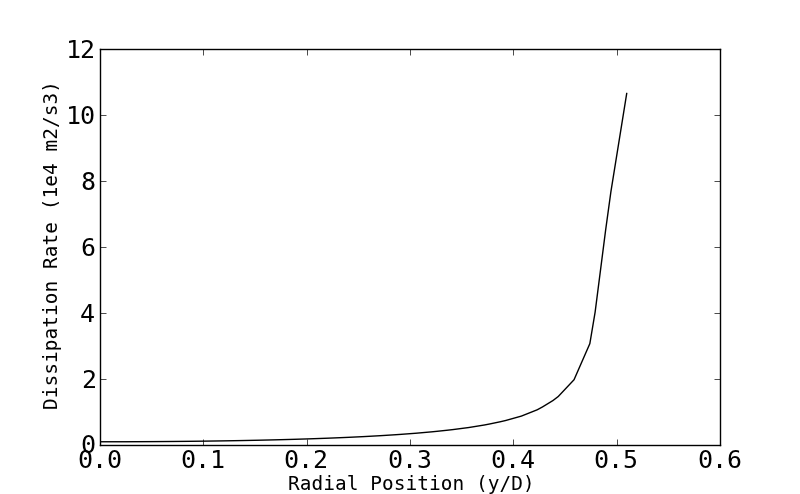
\includegraphics[width=0.5\textwidth]{./figuras/chap3/bc/bc_eps.png}} 
\end{tabular}
 \caption{Radial profiles of the boundary conditions for the gas phase at the nozzle exit plane: mean axial velocity (a), turbulent kinetic energy (b) and its dissipation rate (c).}
 \label{fig: bc_gas}
\end{figure}

\FloatBarrier
\subsection{Coflow}

In the co-flow boundary, only the gas phase is present.

\begin{description}
  \item[Velocity ($\tilde{\bv{U}}_{co-flow}$), Turbulent KE ($k_{co-flow}$) and Dissipation Rate ($\epsilon_{co-flow}$):] A fixed value for velocity was used with the same relations for turbulence properties from \cite{luppes}:
  \begin{equation}
  \begin{split}
  &\tilde{U}_{co-flow} =3\ m/s\, ,\\
   & k =\frac{3}{2} i^2 \bar{U}_{nozzle}^{2}= 0.0054\ J/kg \, , \\
   &\epsilon = \frac{c_{\mu}^{3/4} k^{3/2}}{l_m}=0.0124\ J/kg/s \, ,
  \end{split}
  \end{equation}
  where $\bar{U}_{nozzle}$ is the average velocity in the co-flow region, $i=0.02$ and $l_m = 0.07 D_{co-flow}$.
  
  \item[Temperature ($\tilde{T}_{co-flow}$):] The fixed value of $298\ K$ was used, the ambient temperature.
  \item[Species Concentration ($\tilde{Y}_{k,co-flow}$):] Given the measured mass flow rates of air ($\dot{m}_{air}$) and acetone vapor ($\dot{m}_{ac}$):
  \begin{equation}
  Y_{ac} = 0 \, , \quad Y_{O2} = 0.233 , \quad Y_{N2} = 0.767 \, .
  \end{equation}
  \item[Dynamic Pressure ($p_{d,co-flow}$):] A zero gradient condition was used.
\end{description}

\subsection{Far-field}

Ambient pressure ($p_{\infty}=1\times 10^5\ Pa$) is set for dynamic pressure. Zero gradient is set for the remaining quantities.

\section{Species Equations}

It is only considered the presence of two species: acetone vapor and air. Equation \eqref{av: species1} for the mean mass concentration of acetone vapor ($\tilde{Y}_{ac}$) is then
\begin{equation}
 \frac{\partial \bar{\rho} \tilde{Y}_{ac} }{\partial t} + \nabla
\cdot\left(\bar{\rho} \tilde{\bv{U}} \tilde{Y}_{ac} \right) = \nabla \cdot \left[ \bar{\rho} \left( \nu + \nu_T \right)
\nabla \tilde{Y}_{ac} \right] +\bar{S}_{Yac} \, ,
\end{equation}
The acetone vapor is the scarce species relative to air,
\begin{equation}
\tilde{Y}_{air} = \tilde{Y}_{O2} + \tilde{Y}_{N2}= 1- \tilde{Y}_{ac} \, .
\end{equation}
